% !TeX program = pdflatex   (xelatex and lualatex also work)
%
% Build:  pdflatex memory_module_en.tex   (run twice for the ToC/refs)
% Figures: python ../report/make_figures.py   -> report/fig/*.pdf
%
\documentclass[11pt, a4paper]{article}

\usepackage[T1]{fontenc}
\usepackage[utf8]{inputenc}
\usepackage{lmodern}
\usepackage[margin=2.5cm]{geometry}
\usepackage{booktabs}
\usepackage{longtable}
\usepackage{amsmath, amssymb}
\usepackage{graphicx}
\usepackage{xcolor}
\usepackage[colorlinks=true, linkcolor=blue!50!black, urlcolor=blue!50!black]{hyperref}
\usepackage{enumitem}
\usepackage{fancyhdr}
\usepackage{caption}
\usepackage{microtype}

\graphicspath{{fig/}}
\captionsetup{font=small, labelfont=bf, width=.94\textwidth}
\setlist[itemize]{itemsep=2pt, topsep=3pt}
\setlist[enumerate]{itemsep=2pt, topsep=3pt}

\pagestyle{fancy}
\fancyhf{}
\fancyhead[L]{\small A Separable Memory Module for a Frozen 29M Transformer}
\fancyhead[R]{\small \thepage}
\renewcommand{\headrulewidth}{0.4pt}

\newcommand{\PASS}{\textcolor{green!45!black}{\textbf{PASS}}}
\newcommand{\FAIL}{\textcolor{red!70!black}{\textbf{FAIL}}}
\newcommand{\INVALID}{\textcolor{orange!80!black}{\textbf{INVALID}}}
\newcommand{\SEALED}{\textcolor{blue!60!black}{\textbf{SEALED}}}
\newcommand{\dm}{\Delta m}
\newcommand{\mtext}{m_{\mathrm{text}}}

\title{\textbf{A Separable Memory Module for a Frozen Transformer}\\[5pt]
\large An empirical test of \emph{capability $=$ reasoning $\times$ knowledge}\\
on a 29M-parameter backbone}
\author{MiniMind research fork\\
\small Two-agent protocol: an implementing agent and an adversarial reviewing agent}
\date{4 August 2026}

\begin{document}
\maketitle

\begin{abstract}
\noindent
We report a sequence of controlled experiments on a \textbf{frozen} 29M-parameter
language model, testing whether capability decomposes into \emph{reasoning} and
\emph{knowledge}, and whether the knowledge half can be externalised into a
\textbf{separable, swappable} module.

We build the full pipeline --- event $\to$ write $\to$ store $\to$ retrieve $\to$
deliver $\to$ answer --- and validate it component by component on $S_5$ permutation
composition, whose word problem is NC$^1$-complete.

\textbf{Positive results.} (i) A writer that has never seen the delivery interface
learns, from downstream answer loss alone, to form a latent that the interface consumes
\emph{exactly} (99.0\% on unseen permutations, reconstructing the target encoding to
within $10^{-3}$), while delivery itself costs 1.13M parameters and is precomputable
offline. (ii) The closed loop reaches 98.2\%, exactly the executor ceiling ---
\textbf{integration is free on the answerable path}, and the store round-trip is
numerically free. (iii) Accuracy is \textbf{decoupled from prompt length}: after 128
intervening events memory holds at 100\% while the same information left in context
collapses to 0\%, at $12$--$22\times$ lower per-query prompt cost.

\textbf{Negative results.} (i) Open-set abstention calibration \textbf{does not
transfer}: calibration reads 99.3\%, an untouched test set reads 73.3\%; two
pre-registered versions failed and the line is permanently closed. (ii) A delivered
value \textbf{composes worse} than the same value given as text, and the penalty
compounds with the number of composition steps after delivery. Two repair attempts were
ruled \INVALID{} --- the intervention was indistinguishable from the baseline --- rather
than being counted as failures.

\textbf{Methodological findings.} The cleanest results in this work came from
\textbf{moving responsibility out of learned components and back into contracts or
deterministic rules}. Conversely, \emph{every} mechanistic hypothesis proposed by the
implementing agent was later refuted by measurement. We document how pre-registration,
utility gates, one-sided confidence bounds, and identifiability gates intercepted each
over-claim, including two cases where an early ``100\%'' was merely underpowered.
\end{abstract}

\tableofcontents
\newpage

%==============================================================================
\section{The question}
%==============================================================================

\subsection{Hypothesis}

We test the decomposition
\[
\text{capability} \;=\; \text{reasoning depth} \;\times\; \text{knowledge}
\]
under the claim that the knowledge factor can be \emph{fully externalised}. If it holds,
a small backbone need only be good at \emph{reasoning}; knowledge is supplied by an
external module, so the backbone can punch above its parameter class.

For the claim to survive, the module must be (1)~\textbf{deliverable}, (2)~\textbf{retrievable}
with safe abstention, (3)~\textbf{writable} from observed events, and
(4)~\textbf{composable} --- retrieved knowledge must participate in downstream reasoning,
not merely be read out. We test all four.

\subsection{Why the backbone is frozen}

The backbone is frozen in every experiment. This is deliberate: if the backbone were
allowed to co-train, ``the module is separable'' would be untestable, because we could
not distinguish the module adapting to the backbone from the backbone adapting to the
module. Freezing it makes any success attributable to \textbf{the interface}.

\subsection{Why $S_5$ permutation composition}

The task went through three versions; the first two were invalid and their conclusions
retracted (\S\ref{sec:retract}).

\begin{table}[h]
\centering\small
\begin{tabular}{lccp{7.4cm}}
\toprule
Task & Non-commutative? & Entropy preserved? & Verdict \\
\midrule
mixed arithmetic $(+-\times)$ & yes & \textbf{no}, $3.08 \to 0.62$ bit
  & long chains reward guessing; multiply-only accuracy \emph{rose} with depth \\
add/sub only & \textbf{no} (collapses to $v_0 + \sum \pm r$) & yes
  & a sum is one attention layer (TC$^0$); 8 layers scored 90\% at $k{=}12$ \\
\textbf{$S_5$ composition} & yes & yes (bijections preserve uniformity) & \textbf{current} \\
\bottomrule
\end{tabular}
\end{table}

$S_5$'s word problem is \textbf{NC$^1$-complete}, so a fixed-depth transformer
($\approx$TC$^0$) provably cannot solve arbitrary lengths, whereas addition sits inside
TC$^0$ --- exactly why the add/sub version showed no ceiling at all.

\begin{figure}[h]
\centering
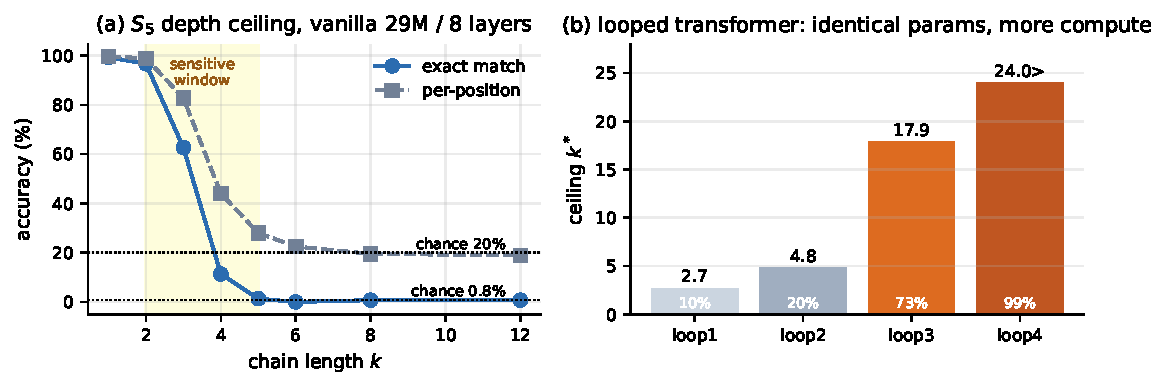
\includegraphics[width=\textwidth]{depth}
\caption{\textbf{(a)} The measured depth ceiling on $S_5$ for the vanilla 29M backbone
(512d / 8 layers / 8 heads / 2 KV heads), 6k steps. Exact-match chance is $1/120=0.8\%$,
per-position chance is 20\%. \textbf{The ceiling is $k \approx 3$ and by $k{=}5$ it is at
chance} --- roughly 2.5 layers per composition step. The sensitive window for any
depth-adding mechanism is $k \in [2,5]$.
\textbf{(b)} Looped transformers, all four from one shared checkpoint, with loop2/3/4
carrying \emph{identical} parameter counts (29.50M) so only compute differs. Bars show
the fitted ceiling $k^*$; the inset percentage is overall accuracy.
\textbf{$+0.9\%$ parameters bought $>9\times$ reasoning depth}, at $3\times$ VRAM. The
jump is super-linear and not smooth: loop2$\to$loop3 is $1.5\times$ the compute for
$3.7\times$ the ceiling, with $k^*/\text{steps}$ moving $0.30 \to 0.75$, suggesting a
phase transition in strategy.}
\end{figure}

All memory experiments below use the \textbf{loop2} backbone (16 sequential steps),
whose single-pass ceiling is $k^* \approx 4.83$.

%==============================================================================
\section{Methodological discipline}\label{sec:method}
%==============================================================================

The work used a two-agent protocol: an implementing agent designed and ran experiments;
a reviewing agent locked the reading rules \emph{before} results were visible. The
following disciplines changed conclusions in several places and are therefore part of
the result.

\begin{description}[leftmargin=1.4em, style=nextline]
\item[Pre-registration.] Reading rules, gates, data identities and checksums, and the
\emph{handling of failure} are written to disk before the run. Locked thresholds are
never revised after seeing results.

\item[Utility gates.] A risk cap alone is passed by the degenerate ``always abstain''
solution. Every safety experiment therefore carries a risk gate \emph{and} a utility
gate. This intercepted a result that would otherwise have looked perfect
(\S\ref{sec:g2c}).

\item[Bounds, not point estimates.] Zero errors in a small sample is not low risk. All
hallucination rates are reported with a \textbf{one-sided 95\% Clopper--Pearson upper
bound}. This is how we discovered that an earlier ``100\% hit/miss'' was merely
underpowered (\S\ref{sec:g3e}).

\item[Identifiability gates.] An intervention must first be shown \emph{distinguishable
from the baseline} before long training is justified. This caught two invalid
specifications (\S\ref{sec:g6}).

\item[Never backfill a milestone.] Failed pre-registered results are permanent. Later
versions get new names and new sections and may not retroactively convert an old
\FAIL{} into a \PASS{}.
\end{description}

%==============================================================================
\section{Infrastructure}
%==============================================================================

\subsection{Canonical key spans}

The custom 6400-token BPE vocabulary tokenises \textbf{context-dependently}:
\verb|"f0"| $\to$ \verb|[105,51]| but \verb|" f0"| $\to$ \verb|[341,51]|. Keys always
appear with a leading space in every view, so the canonical form must include it.

Measuring with the bare form reported \textbf{28 pairs of ``identical'' hidden states}
and produced a wrong claim. With the corrected span only 7 pairs remain, and their raw
$\max|\text{diff}|$ is $6\times10^{-2}$ to $1.5\times10^{-1}$ against $\|h\| = 41.3$ ---
\textbf{not exact overlap at all}. Since then \verb|canonical_key_ids| and
\verb|locate_key_span| are the single source of truth and every symbol-identity
comparison must route through them.

\subsection{Data-integrity gates}

Each of these exists because it once produced a wrong conclusion:

\begin{itemize}
\item \textbf{Never skip rows silently.} Dropping over-long samples does not thin a
dataset uniformly --- it removes the \emph{deepest} samples first, exactly the range a
depth experiment measures. Now counted per $k$ and raised.
\item \textbf{A matched comparison needs a fingerprint, not a shared seed.} Three
conditions built from ``the same seed'' are only \emph{argued} to be identical. We hash a
canonical latent stream that never reaches the model, and verify the hash changes with
the seed (a constant hash also ``matches'').
\item \textbf{Deduplicate on what the model can see.} Two different sample identifiers
can render to identical visible content; keying on the render-level identifier caught a
real cross-split leak.
\end{itemize}

%==============================================================================
\section{G1: delivery}
%==============================================================================

A frozen backbone trained on explicit values ($L_0$, 100\%) must instead consume a
25-dimensional lossless latent supplied by a learned adapter. Selection is oracle and
the store is frozen, so \textbf{only delivery is under test} and a failure localises.

\begin{figure}[h]
\centering
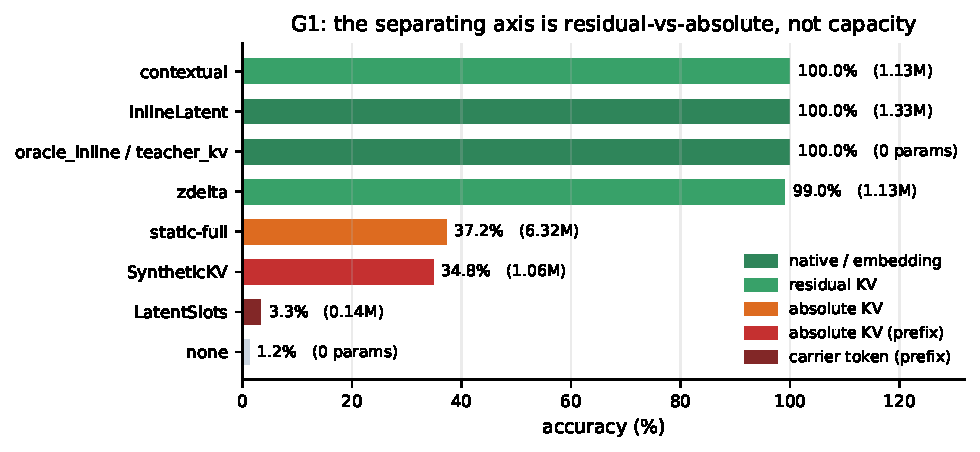
\includegraphics[width=.9\textwidth]{delivery}
\caption{Eight delivery mechanisms. The separating axis is \textbf{residual versus
absolute}, not capacity and not position: a \textbf{6.32M} absolute-KV adapter fails
(37.2\%) where a \textbf{1.13M} residual one succeeds (99.0\%). Delivering the latent as
an embedding at the value positions, or as a residual correction to the native KV, both
reach 100\%; writing an absolute KV, or prefixing carrier tokens, does not.}
\end{figure}

\subsection{What holds}

A frozen backbone \emph{can} consume learned latent delivery at 100\%, as an
\textbf{embedding at the value positions} or as a \textbf{residual KV correction}.
Delivery is an embedding or a KV --- \textbf{not text}. The intuition that ``memory must
enter as tokens'' is false.

\subsection{The sealed interface}

The default interface for all later stages is \verb|zdelta|:
\[
K' \;=\; K_{\mathrm{native}} \;+\; f_{\mathrm{slot}}(z)
\]
at the value token positions, across all 16 (loop, layer) cache slots; 1.13M parameters,
backbone frozen, 99.0\%. Crucially $f(z)$ is \textbf{computable offline after retrieval},
so only the native scaffold forward pass and a per-position addition are online.

\subsection{Retracted here}

Three claims held earlier and now permanently withdrawn: delivery must be
just-in-time/streaming (refuted by a padded variant at 100\%); memory must flow through
the backbone (\verb|zdelta| injects per layer and scores 99.0\%); the synthesiser must
see the layer state (\verb|zdelta| has no context input).

%==============================================================================
\section{G2: retrieval}
%==============================================================================

\begin{table}[h]
\centering\small
\begin{tabular}{llll}
\toprule
Stage & Address source & Key identities & Result \\
\midrule
G2a & fixed random orthogonal & fixed \verb|f0..f3| & 100\% ordered / per-step / hit-miss$^\dagger$ \\
G2b & same, query from frozen backbone hidden & fixed & 100\%$^\dagger$ \\
G2c & \textbf{tied encoder over canonical key spans} & \textbf{disjoint splits}
  & retrieval \textbf{98.1\%}, hit/miss \textbf{73.3\% / 81.5\%} \\
\bottomrule
\end{tabular}
\end{table}

$^\dagger$\,\textbf{This 100\% is underpowered}; see \S\ref{sec:g3e}.

\subsection{G2c: a split result}\label{sec:g2c}

\textbf{What transfers.} Unseen-identity \emph{ranking}: per-step recall 98.1\% on both
seeds, with the encoder pushing input-side $\max|\cos|$ from 0.964 apart to 0.824.

\textbf{What does not.} A single support \textbf{threshold}. Calibration reads
99.3--99.5\%; the untouched test set reads 73.3--81.5\%. Diagnosis shows the \emph{score}
separates --- an oracle threshold reaches 96.3--98.0\% --- so the entire gap is threshold
placement:

\begin{table}[h]
\centering\small
\begin{tabular}{llrrrrr}
\toprule
Seed & Set & Frozen thr. & Oracle upper & Gap & Steps with $\cos>0.8$ & Accuracy there \\
\midrule
42 & TRAIN & 100.0\% & 100.0\% & 0.0\% & 0 & --- \\
42 & CAL & 99.6\% & 99.6\% & 0.0\% & \textbf{0} & --- \\
42 & TEST & 73.5\% & \textbf{96.3\%} & \textbf{22.8\%} & 269 & 9.7\% \\
43 & CAL & 99.5\% & 99.5\% & 0.0\% & \textbf{182} & \textbf{100.0\%} \\
43 & TEST & 84.6\% & \textbf{98.0\%} & \textbf{13.4\%} & 153 & 9.8\% \\
\bottomrule
\end{tabular}
\end{table}

\subsection{A hypothesis withdrawn mid-experiment}

We briefly concluded that the calibration set lacked hard cases --- seed 42's calibration
set indeed has no pair above 0.8. \textbf{Seed 43 refutes it}: its calibration set
contains 182 hard steps, all correct under the frozen threshold, while the same threshold
scores 9.8\% on the test set's 153 hard steps. \textbf{The score's scale moves with the
identity set; it is not a coverage problem.} The bin-based inclusion rule we derived from
that hypothesis was withdrawn too: the 0.8 boundary was chosen \emph{after seeing where
the test set broke}, so using it to select calibration data would degrade the fix into
hard-negative curation.

\subsection{G2c-cal-v2: \FAIL{}, permanently}

One pre-registered re-calibration on 40 brand-new identities, both seeds:

\begin{table}[h]
\centering\small
\begin{tabular}{lrr}
\toprule
& Seed 42 & Seed 43 \\
\midrule
Calibration missing cases & 122 (zero-error UB 2.4\%) & 126 (2.3\%) \\
Selected threshold & $+16.985$ & $+16.295$ \\
\textbf{Minimum achievable false-abstain on calibration} & \textbf{98.1\%} & \textbf{97.6\%} \\
Test hallucination, one-sided 95\% UB & 2.9\% \PASS{} & \textbf{6.6\%} \FAIL{} \\
Test false-abstain & \textbf{97.3\%} \FAIL{} & \textbf{98.2\%} \FAIL{} \\
\bottomrule
\end{tabular}
\end{table}

\textbf{The utility gate is what caught it.} Subject to a one-sided 95\% bound on
hallucination $\le 5\%$, the \emph{minimum achievable} false-abstain \emph{on the
calibration set} was already 98\%. \textbf{Without that gate this would have passed
looking like ``R\_abstain 100\%, hallucination 0\%''} --- a threshold that always
abstains. The line is closed: no third version, no length-conditioned threshold, no
rebalanced retraining.

\textbf{Confound.} The v2 identity sets are almost all 3-token spans while training
identities are almost all 2-token, so the failure occurs under a \textbf{joint identity
and span-structure shift}, and this design cannot separate the two. Recorded as design
debt: a canonical encoder's training must cover the tokenisation structure it will meet.

%==============================================================================
\section{G3: write, closure, faults, boundaries, safety}
%==============================================================================

\subsection{G3a: write formation}

Can a writer form, from an \emph{event}, a latent that a \textbf{frozen, independently
trained} delivery interface consumes? The writer has never seen \verb|zdelta| and
\verb|zdelta| has never seen the writer. Events look like \verb :| f3 = 3 1 0 2 4: ,
deliberately containing no chain and no state. The generalisation axis is the
\textbf{permutation} (95 train / 24 val, disjoint), not key identity.

\begin{table}[h]
\centering\small
\begin{tabular}{lrrrrr}
\toprule
Version & writer output & end-to-end (unseen perms) & row argmax & valid perm & latent dist. \\
\midrule
oracle & \verb|perm_to_latent| & \textbf{99.0\%} & --- & --- & 0 \\
\textbf{v1} & unconstrained 25-d & \textbf{3.5\%} \FAIL{} & 37.1\% & 0.0\% & 2.32 \\
\textbf{v2} & \textbf{$5\times5$ row softmax} & \textbf{99.0\%} \PASS{} & \textbf{100\%}
  & \textbf{100\%} & \textbf{0.001} \\
zero / shuffled & --- & 0.5\% / 0.8\% & --- & --- & --- \\
\bottomrule
\end{tabular}
\end{table}

\textbf{v2 matches the oracle cell for cell}, and reconstructs \verb|perm_to_latent| to
within $0.001$ --- having \textbf{never been supervised on that encoding}, only on
downstream answer loss.

\textbf{End-to-end alone cannot read this.} v1's row-argmax is 37.1\% against 20\%
chance: partial formation, entirely invisible in a 3.5\% end-to-end number.

\textbf{What may be claimed.} A row-categorical parameterisation makes task-loss-only
write formation \emph{optimisable}. Row softmax guarantees only that each row is
non-negative and sums to one; the 100\% valid-permutation rate and 0.005 row entropy are
\textbf{learned}, not structural --- which makes the result stronger, not weaker.

\textbf{What may not.} Do not attribute this to manifold mismatch alone: v1$\to$v2
changed the output constraint \emph{and} the gradient geometry. Do not say it ``emerges
without priors''; the conclusion is scoped to the known $S_5$ latent schema.

\subsection{G3b: closure}

All four components loaded frozen, \textbf{zero training}, wired as event $\to$ writer
$\to$ commit $\to$ retrieve $\to$ read $\to$ deliver $\to$ answer; 400 episodes.

\textbf{Scope, stated not implied}: only \textbf{4 query identities} and at most
\textbf{32 orthogonal addresses}. Addresses still come from a known key rule, so
\textbf{write-address formation is untested here}.

\begin{figure}[h]
\centering
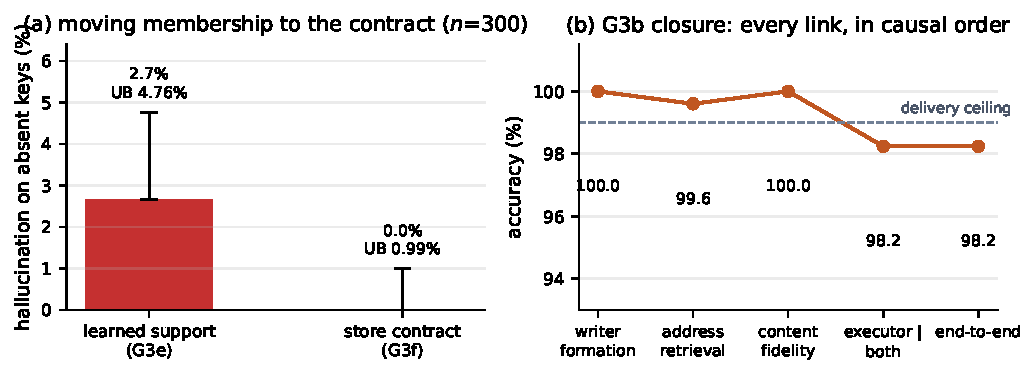
\includegraphics[width=\textwidth]{safety}
\caption{\textbf{(a)} Moving membership from a learned support head to a store contract.
On the \emph{identical} 300 missing episodes, the learned head hallucinates 8/300
(2.7\%, UB 4.76\%); the contract hallucinates \textbf{0/300} (UB 0.99\%) while leaving
utility untouched ($A_{\mathrm{ans}}$ 100\%, false-abstain 0/300). Error bars are
one-sided 95\% Clopper--Pearson upper bounds.
\textbf{(b)} The G3b causal chain in order. Formation and content fidelity are exact; the
1.8\% shortfall at the executor equals the delivery ceiling (dashed), so it is \emph{not}
an integration loss.}
\end{figure}

\begin{table}[h]
\centering\small
\begin{tabular}{lrr}
\toprule
Chain step & primary (2-token) & stress (3-token, exploratory) \\
\midrule
1. writer formation exact (\textbf{unconditional}) & \textbf{100.0\%} ($n{=}904$) & 95.7\% ($n{=}897$) \\
2. address retrieval exact & \textbf{99.6\%} ($n{=}1000$) & \textbf{7.9\%} ($n{=}1000$) \\
3. retrieved-content fidelity $\mid$ address correct & \textbf{100.0\%} ($n{=}904$) & --- \\
4. executor $\mid$ address $+$ content correct & \textbf{98.2\%} ($n{=}341$) & --- \\
5. \textbf{end-to-end} & \textbf{98.2\%} ($n{=}341$) & \textbf{0.0\%} ($n{=}339$) \\
R\_abstain / halluc. / false-abstain & 94.9\% / 5.1\% / 0.0\% & 90.2\% / 9.8\% / 85.5\% \\
\bottomrule
\end{tabular}
\end{table}

\textbf{On the answerable path, integration costs nothing.} Every cell of the $2\times2$
intervention (oracle$\mid$learned writer $\times$ oracle$\mid$learned retrieval) scores
\textbf{98.2\%} end-to-end, \emph{including} oracle$\times$oracle --- so the missing 1.8\%
is a shared executor ceiling and not an integration loss. Direct delivery and store
round-trip are identical, so the round-trip is numerically free. The store contract was
verified bitwise over 3200 commit$\to$read pairs: shape 3200/3200, $\max|\text{diff}|$
$0.00\mathrm{e}{+}00$, detached 3200/3200, address$\leftrightarrow$content binding 3200/3200.

\textbf{But do not generalise to ``integration is free''.} Abstention is the one cell that
moves (oracle retrieval 100\% vs.\ learned 94.9\%), placing \textbf{3/59 $=$ 5.1\%
hallucination} entirely on the learned support head. \textbf{That number is not folded
into the \PASS{}.} Three claims, none cancelling the others: in-distribution 2-token
answerable closure \PASS{}; missing safety \emph{not cleanly reliable}; 3-token
span-shift robustness \FAIL{}.

\subsection{G3c: storage fault injection --- \SEALED{}}

Pin the contract first --- \emph{address visible} $\Leftrightarrow$ \emph{committed
content readable}, atomic commit --- then break it on purpose. On an inconsistent read
the controller must \textbf{fail closed} to abstain.

\begin{table}[h]
\centering\small
\begin{tabular}{llrrr}
\toprule
Injection & fail-closed & answered & correct $\mid$ answered & \textbf{hallucination} \\
\midrule
\verb|none| & yes & \textbf{100.0\%} & \textbf{99.2\%} & 0.0\% ($n{=}0$) \\
\verb|dangling| & yes & 0.0\% & --- & \textbf{0.0\%} ($n{=}240$) \\
\verb|torn_commit| & yes & 0.0\% & --- & \textbf{0.0\%} ($n{=}240$) \\
\verb|stale| & yes & 0.0\% & --- & \textbf{0.0\%} ($n{=}240$) \\
\verb|dangling| & \textbf{no (control)} & 100.0\% & 0.8\% & \textbf{100.0\%} \\
\verb|torn_commit| & \textbf{no (control)} & 100.0\% & 11.2\% & \textbf{100.0\%} \\
\verb|stale| & \textbf{no (control)} & 100.0\% & 7.9\% & \textbf{100.0\%} \\
\bottomrule
\end{tabular}
\end{table}

Two things must hold together to seal: hallucination is zero under the guard,
\textbf{and} the \verb|none| baseline answers 100\% at 99.2\% correct --- the guard
\textbf{does not over-trigger}, so it is not another ``always abstain'' degenerate. Here
\emph{hallucination} means \textbf{answering while having read corrupted content}; being
accidentally right is still unsafe.

Two things we had to fix in the process. The \verb|stale| injection initially changed
only the version metadata, so the unguarded control still answered 100\% correctly ---
proving only that the version check was wired, not that it blocked any harm; injecting a
\emph{divergent} old value dropped the control to 7.9\%. And the wrong-key branch never
fired in natural evaluation, which shows only that the retriever never picked wrongly ---
\textbf{it does not show the fail-closed branch works}. A deliberate injection of 60
mismatched reads yielded \textbf{0/60} deliveries; only then was contract~C exercised.

\subsection{G3d: boundary audit}

Two \textbf{single-variable}, fully frozen sweeps, with no recalibration. Attribution on
the $k$ axis needs \textbf{three rows}, not two: the \verb|oracle+zdelta| row \emph{still}
passes through a \verb|zdelta| trained only at $k \le 4$, so an $L_0$ row (values in the
prompt, no delivery at all) is required to separate executor from delivery.

\begin{figure}[h]
\centering
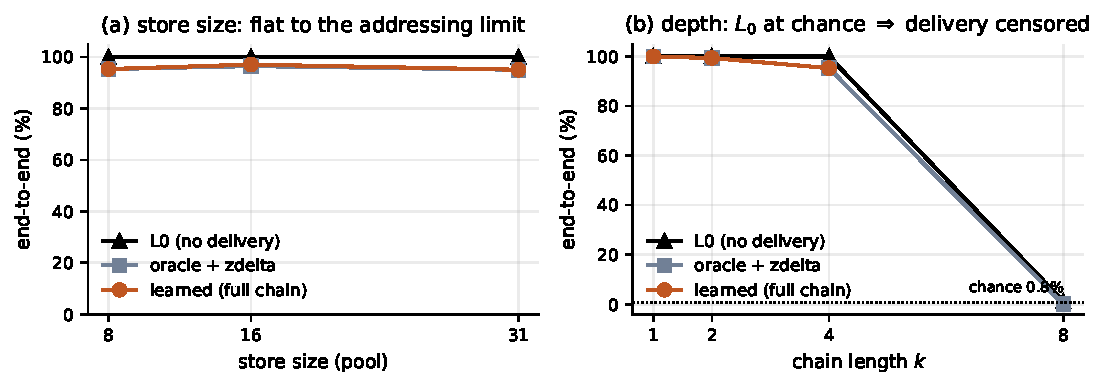
\includegraphics[width=\textwidth]{boundary}
\caption{\textbf{(a)} Store size is not the bottleneck: 8 $\to$ 31 entries is flat, with
$R_{\mathrm{abstain}}$ 100\% and hallucination 0\% throughout. 31 is the testable maximum
--- an omitted-write episode needs 31 in the pool \emph{plus} one omitted, and the omitted
key must not remain addressable.
\textbf{(b)} Depth. At $k{=}8$ the $L_0$ row is at 1.1\%, i.e.\ \textbf{chance} (0.83\%).
The delivery result there is therefore \textbf{censored by the backbone ceiling}: the cell
supports \emph{neither} \verb|zdelta| failing \emph{nor} succeeding. The only citable
positive statement is that this backbone has no usable executor headroom at $k{=}8$.}
\end{figure}

Establishing that pool size is the \emph{only} varying factor took two independent pieces
of evidence, and one is not enough: (i) distractors were selected \textbf{0 times}, so
their content cannot have reached the executor; (ii) a \textbf{label-swap invariance} test
over 120 episodes found retrieval logits and support scores identical to
$0.000\mathrm{e}{+}00$ with zero decision or top-1 mismatches. Evidence (i) alone is
insufficient because the support head reads the \emph{whole} logit geometry (top-1,
top-1 $-$ top-2, logsumexp), so an address that never becomes top-1 can still move the
threshold decision.

\subsection{G3e: replicating a safety number}\label{sec:g3e}

Hallucination counts of 2/32 and 3/59 were already two small-sample non-zeros, so we ran a
single pre-registered \textbf{stratified} replication: 300 missing $+$ 300 answerable,
fully frozen, no recalibration, no seed selection, no re-runs.

\begin{table}[h]
\centering\small
\begin{tabular}{lr}
\toprule
Missing condition ($n{=}300$) & \\
\midrule
$R_{\mathrm{abstain}}$ & 97.3\% [94.8\%, 98.6\%] \\
\textbf{hallucination} & \textbf{2.7\% (8/300)}, \textbf{one-sided 95\% CP upper bound 4.76\%} \\
\midrule
Answerable condition ($n{=}300$) & \\
\midrule
$A_{\mathrm{ans}}$ & \textbf{100.0\%} [98.7\%, 100.0\%] \\
false-abstain & \textbf{0.0\%} [0.0\%, 1.3\%] \\
\bottomrule
\end{tabular}
\end{table}

Three independent measurements agree in direction (2/32, 3/59, 8/300): the closed-world
support head has a \textbf{rare but real} failure mode.

\textbf{This forces a correction to an earlier number.} G2a/G2b's ``hit/miss 100\%'' was
\textbf{underpowered}: those runs saw about 60 missing cases, and
$P(0 \mid n{=}60,\, p{=}0.027) \approx 0.19$ --- entirely compatible with a true rate of
2.7\%. The observation stands; the \emph{interpretation} that support was perfect does not.

\subsection{G3f: membership belongs to the contract --- \SEALED{}}

In this task the query carries a canonical exact key and the store commits under that same
key, so $\texttt{contains}(key)$ is a \textbf{decidable data-structure fact}. Asking a
learned similarity to guess it is a category error; moving it back is \textbf{correct
typing, not evasion}.

The authoritative path is $\text{canonicalize}(key) \to \texttt{store.contains}(key)$:
absent \textbf{hard-abstains} before retrieval is even permitted; present proceeds; after
the read the entry's key and committed content are asserted or the controller fails
closed. The learned support survives only as a \textbf{shadow metric} and may never
override the guard.

On the \emph{identical} episodes the shadow column reproduces exactly the \textbf{8/300}
it would have let through (Figure~3a). That is a controlled demonstration that the guard
removed \emph{those} failures, not that it drew an easier sample.

\textbf{What this does not fix.} The open-set semantic problem is untouched: with no
reliable canonical key, a key-extraction error, or a ``semantically related'' rather than
same-ID lookup, the store cannot answer. \textbf{G2c's calibration failure remains a
whole-system blocker and is not backfilled.}

%==============================================================================
\section{G4: addressing and temporal binding}
%==============================================================================

\subsection{G4a: write-address plumbing --- \PASS{}}

The responsibility split is the point: the \textbf{writer forms content $z$ only} (it
never emits a membership bit), a key extractor handles the literal key, and the
\textbf{store owns atomic binding and membership}. The address is
\verb|address_vector(key)| --- \textbf{zero learned parameters}. We deliberately do
\emph{not} train an MLP to ``learn addresses'' over a handful of closed keys and call it
formation; that is a lookup table, and a deterministic map is the more honest statement.

With \textbf{25 unseen 2-token identities} and \textbf{key$\leftrightarrow$permutation
re-paired at random every episode}: key extraction exact \textbf{100.0\%} (3200/3200);
address$\leftrightarrow$content binding \textbf{100.0\%} (3200/3200); missing
$R_{\mathrm{abstain}}$ 100.0\% and hallucination \textbf{0/200} (UB 1.49\%); answerable
$A_{\mathrm{ans}}$ \textbf{100.0\%}, false-abstain 0.0\%.

This proves only that \emph{usable entries can be created}. It does not prove semantic
binding, content addressing, or generalisation across span structures.

\subsection{G4b: temporal / referential binding}

Events form an \textbf{ordered stream}; the query uses a \textbf{reference} (``the
previous one'' $=$ the most recently written entity) rather than a literal key.

\textbf{The reference must sit on the read side.} The membership guard of \S G3f blocks
only \emph{non-existent} keys; it cannot block a resolver pointing at \emph{another
existing} entity --- that key really is in the store, the guard passes, and the system
\textbf{confidently delivers the wrong content}. Hence \emph{wrong-existing-entity} is
this stage's only dangerous error, reported separately from abstention.

\textbf{The oracle rung earned its keep.} The first oracle ceiling came out at
\textbf{0.0\%} --- because the stream prefix and reference suffix had been placed inside
the \emph{delivery} prompt, which the frozen backbone had never seen in that shape. This
violated an invariant established earlier: the reference/retrieval view must be
out-of-band, and the delivery prompt must not change. With an independent reference view,
all nine cells (2/3/5 entities $\times$ 0/2/5 fillers) reach \textbf{100\%}. \textbf{Had
this error been mixed into a learned resolver, it would have presented as ``temporal
binding cannot be learned'', with a cause unrelated to binding.}

\begin{table}[h]
\centering\small
\begin{tabular}{lrr}
\toprule
& A (single last-token summary) & \textbf{B (candidate-wise readout)} \\
\midrule
probe train / test & 44.7\% / \textbf{34.8\%} (chance 34.4\%) & \textbf{100\% / 100\%} \\
formal test, raw exact & --- & \textbf{94.5\%} (harder split) \\
\bottomrule
\end{tabular}
\end{table}

\textbf{The recency information is in the per-entity hidden states, but not in a single
last-token summary.} A is permanently recorded as a \emph{final-token/final-layer linear
readout} \FAIL{} and is \emph{not} superseded by B.

The pre-locked selective policy (calibration picks the threshold whose one-sided 95\% bound
on wrong-existing-entity is $\le 5\%$, then minimises abstention; test runs once) gives
coverage 84.8\%, abstention 15.2\%, and guarded wrong-existing 8/509 $=$ \textbf{1.6\%}
(UB 2.82\%) $\Rightarrow$ \PASS{}.

\textbf{But the honest headline is that the learned version loses to a rule that needs no
learning.} The non-learned $\arg\max(\text{last write position})$ baseline is
\textbf{100.0\%}, against 94.5\% raw for the learned resolver, and B is almost certainly
just \emph{reading position} --- each entity's hidden state carries its sequence position
by construction. The claim is therefore capped at ``a candidate-wise temporal resolver /
controller readout is feasible'', and explicitly not at neural working memory.

%==============================================================================
\section{G5: what memory actually buys}
%==============================================================================

\subsection{G5a: information retention / context extension --- \PASS{}}

This experiment does \textbf{not} claim reasoning improves. Five paired conditions, same
backbone, same query, same identities, same items.

\begin{figure}[h]
\centering
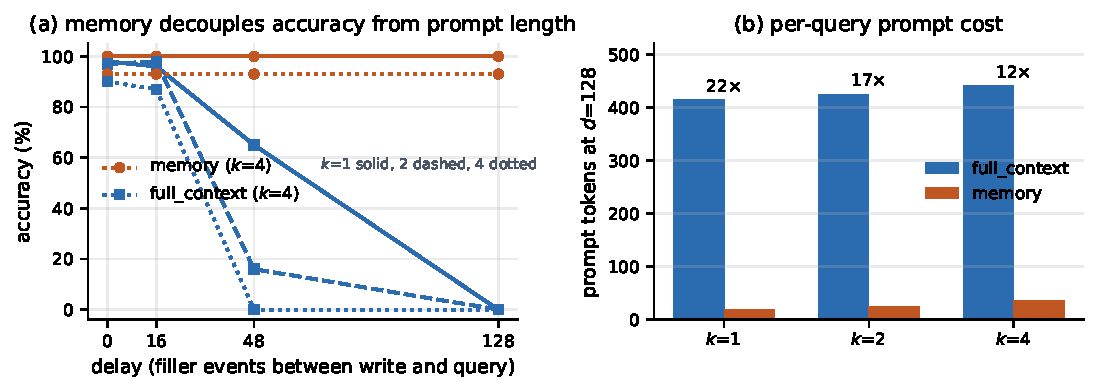
\includegraphics[width=\textwidth]{retention}
\caption{\textbf{(a)} Accuracy against delay (filler events between write and query).
\texttt{memory} is \textbf{flat} at every $k$; \texttt{full\_context} --- the ``keep
everything in the prompt'' alternative --- collapses to 0\%. Overall:
\texttt{oracle\_L0} 100\% $\mid$ \textbf{\texttt{memory} 97.7\%} [96.6, 98.4] $\mid$
\texttt{full\_context} 53.9\% $\mid$ \texttt{shuffled} 6.3\% $\mid$ \texttt{no\_memory}
\textbf{0\%}. The floor and control both collapse, so the score comes from the delivered
content and not from carrier positions.
\textbf{(b)} Per-query prompt cost at the longest delay.}
\end{figure}

\textbf{A sentence that must appear verbatim in the conclusion:} \emph{this result does
not support a comparison between memory and a long-context-trained model; the
\texttt{full\_context} decline is confounded with an $11$--$23\times$ length
distribution shift.} The backbone's \verb|max_position_embeddings| is 1024, so 414 tokens
is \emph{within} range --- but its training prompts were 19--37 tokens, making $d{=}128$
some 11--23$\times$ longer than anything it saw.

\textbf{The cost claim is likewise narrowed:} $12$--$22\times$ is the \textbf{per-query
backbone prompt cost}, \textbf{not} a lifecycle cost --- memory still paid for the writer,
the commit, retrieval, and event processing. Unless writes amortise over many queries, no
end-to-end compute claim follows.

\textbf{What may be claimed:} \emph{memory decouples accuracy from prompt length}. For a
backbone whose usable context is short, that is a large practical gain.

\subsection{G5b--G5c: segmentation, and where memory breaks}

Since $st \leftarrow st \circ p$, starting from the identity and running $p_1..p_j$ yields
the \emph{composed permutation} $P_j$, and $st_0 \circ P_j = st_j$. A checkpoint can
therefore be \textbf{a permutation placed in a value slot} --- exactly the role
\verb|zdelta| was trained for --- so no new interface is needed.

\begin{figure}[h]
\centering
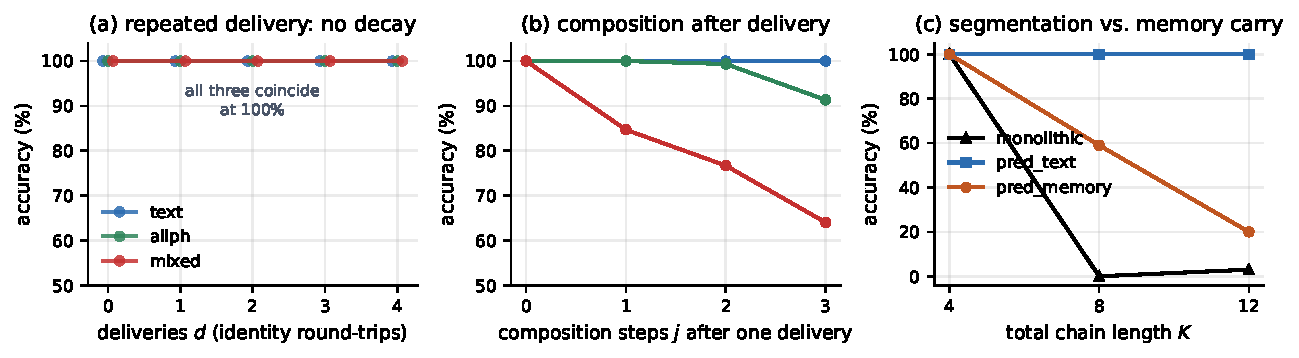
\includegraphics[width=\textwidth]{composition}
\caption{\textbf{(a)} Repeated delivery with a semantic-identity round trip (ground truth
held constant): all three configurations stay at 100\% for $d = 0..4$. There is
\textbf{no per-delivery fidelity loss}, and the mixed configuration alone costs nothing.
\textbf{(b)} One delivery, then $j$ real composition steps. \texttt{text} stays at 100\%
for all $j$, so composition itself is fine; \texttt{allph} decays slowly and
\texttt{mixed} steeply. \textbf{The failure lives in the interaction of delivery with
subsequent composition}, plus an additional, independent penalty for mixed carriers
(15pp at $j{=}1$).
\textbf{(c)} Segmenting a length-$K$ chain into pieces of $\le 4$. \texttt{monolithic}
is at 0\% ($K{=}8$) and 3\% ($K{=}12$); with explicit text checkpoints it is 100\%,
with memory-carried checkpoints it degrades with the number of mixed deliveries.}
\end{figure}

Reading Figure~5c in the pre-locked way:

\begin{itemize}
\item \textcircled{1} vs.\ \textcircled{3}: $0\% \to 100\%$ at $K{=}8$ and $3\% \to
100\%$ at $K{=}12$. Segmentation with explicit checkpoints \textbf{bypasses this
backbone's monolithic chain-length boundary} while every call still runs at $k \le 4$ ---
\textbf{single-pass depth is never exceeded}.
\item \textcircled{2} vs.\ \textcircled{3}: intermediate error propagation is \textbf{zero}.
\item \textcircled{3} vs.\ \textcircled{4}: the loss compounds with the number of mixed
deliveries.
\end{itemize}

\textbf{Strictly, \textcircled{1} vs.\ \textcircled{3} shows that \emph{segmentation}
works, not that \emph{memory} works} --- \textcircled{3} carries checkpoints as plain
text. Memory's value requires \textcircled{4} to catch up with \textcircled{3}. The
permitted phrasing is ``multiple backbone calls plus explicit checkpoints bypass the total
chain length''; not that the single-pass executor became deeper. The two arms differ in
compute, so this is a systems capability/compute trade-off, not an equal-compute model
comparison.

\subsection{G5b confirmatory: \FAIL{}}

An exploratory all-placeholder arm reached 96.7\% ($n{=}60$) --- but it was designed
\emph{after} seeing a smoke run. Re-run with a fresh seed, an untouched split, and
$n{=}100$:

\begin{table}[h]
\centering\small
\begin{tabular}{lrrr}
\toprule
$K$ & \verb|pred_text| & \verb|pred_mem_allph| & gap \\
\midrule
8 & \textbf{100.0\%} & \textbf{84.0\%} & \textbf{$+16.0$pp} \FAIL{} \\
12 & \textbf{100.0\%} & \textbf{81.0\%} & $+19.0$pp \\
\bottomrule
\end{tabular}
\end{table}

The pre-locked gate (memory within 5pp of text \emph{and} $\ge 95\%$ at $K{=}8$) fails on
both counts. \textbf{The exploratory 96.7\% did not replicate.} This is the second
instance of the same lesson (\S\ref{sec:g3e} was the first): \emph{conditions designed
after looking at the data read optimistically}.

%==============================================================================
\section{G6: repair attempts and the complete logit-level account}\label{sec:g6}
%==============================================================================

\subsection{\texttt{zdelta-v2}}

Delivery only is trained; backbone, writer, store and retriever stay frozen. The two
training objectives are \textbf{not} split into two losses --- the same factorial episode
crosses $j$ with the carrier configuration, otherwise the model never sees the cells that
actually fail. Training covers 5 cells; held-out includes a \textbf{$j$ extrapolation}
(train $j \le 2$, test $j{=}3$). \textbf{The primary is ``match text carry'', not ``beat
v1''.}

\begin{figure}[h]
\centering
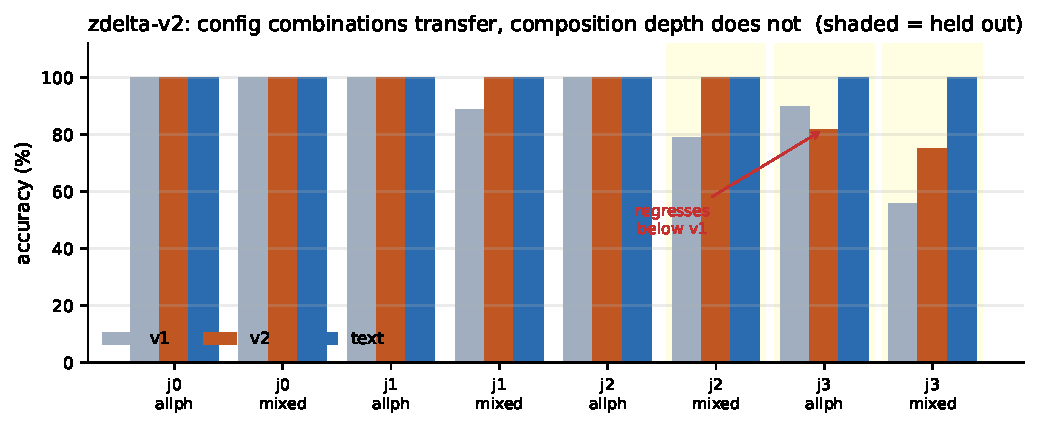
\includegraphics[width=\textwidth]{v2}
\caption{\texttt{zdelta-v2}. Trained cells all reach 100\%. The unseen \emph{configuration}
combination ($j{=}2$ mixed) transfers completely, 79\% $\to$ 100\%. But the unseen
\emph{depth} does not, and $j{=}3$ allph \textbf{regresses below v1} (90\% $\to$ 82\%).
Under the pre-locked reading this is \textbf{finite-horizon coverage repair, not
composition-stable delivery}. Note the narrowing: \emph{configuration combinations
transfer; composition depth does not}.}
\end{figure}

\subsection{Paired logit decomposition}

With teacher forcing we measure, per output position,
\[
\mtext = \mathrm{logit}(\text{correct}) - \max_{\text{wrong}}, \qquad
\dm = m_{\mathrm{delivery}} - \mtext,
\]
so a flip occurs \emph{exactly} when $\mtext + \dm < 0$.

\begin{figure}[h]
\centering
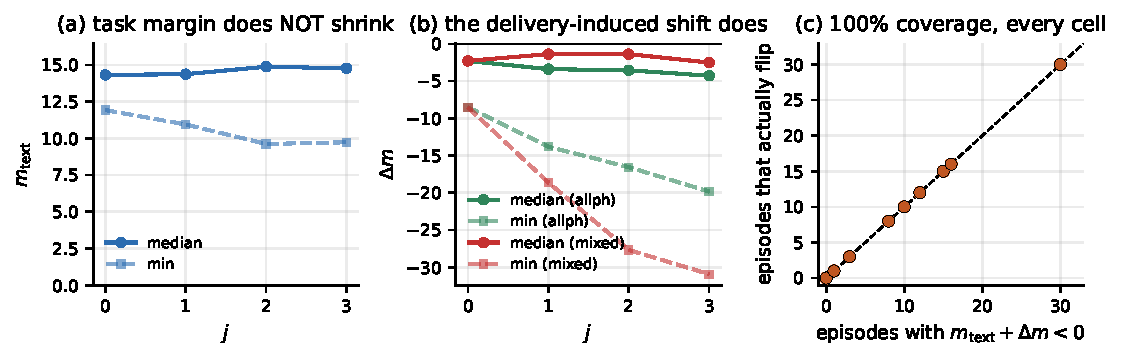
\includegraphics[width=\textwidth]{margin}
\caption{\textbf{(a)} The task margin under text carry does \textbf{not} shrink with
composition depth (median $14.33 \to 14.78$), so the failure cannot be attributed to
rising task difficulty. \textbf{(b)} What degrades is the delivery-induced shift $\dm$,
and its \emph{negative tail} degrades much faster than its median: \texttt{allph}'s median
roughly doubles ($-2.28 \to -4.28$) while \texttt{mixed}'s minimum grows about fourfold
($-8.5 \to -30.9$). \textbf{The mixed penalty is tail risk, not an average effect} --- its
median $\dm$ is in fact milder than \texttt{allph}'s. \textbf{(c)} Predicted flips
($\mtext + \dm < 0$) against observed flips, one point per cell: the accounting closes at
\textbf{100\% coverage in every cell}.}
\end{figure}

The three pre-locked conditions resolve as: (1)~$\mtext$ falls systematically with $j$?
\textbf{No}. (2)~$\dm$'s conditional distribution is $j$-independent? \textbf{No}.
(3)~$\mtext + \dm < 0$ predicts flips? \textbf{Yes, 100\%}. The margin hypothesis is
therefore refuted and the mechanism is a \textbf{task-relevant directional interaction}.

This also explains v2's regression exactly: at $j{=}3$ allph its median $\dm$ moved from
$-4.277$ to $-5.856$, and the count of positions with $\mtext + \dm < 0$ went $10 \to 12$
while the observed flips went $10 \to 12$ --- \textbf{finite-horizon overfitting reconciled
item by item at the logit level}.

\subsection{Two invalid specifications}

\begin{itemize}
\item \texttt{v3-hinge}: \INVALID{} / no effective intervention. A per-position hinge
$\max(0, \varepsilon - m_{\mathrm{delivery}})$ with $\varepsilon = 8.0$ locked in advance
produced \textbf{$\text{hinge} = 0.0000$ throughout training} --- margins in the training
cells already exceed 8. The loss was effectively v2's plain cross-entropy.
\item \texttt{v3-distill} ($T{=}1$): \INVALID{} / indistinguishable from cross-entropy.
\textbf{KL equalled CE on every row}, for a mathematical reason: the text teacher's margin
is about 14, so its distribution is effectively one-hot and
$\mathrm{KL}(\text{one-hot} \,\|\, \text{student}) = -\log p_{\text{student}}(\text{gold})
= \mathrm{CE}$. Setting $\lambda_{\mathrm{KL}} = 1$ merely doubled the cross-entropy.
\end{itemize}

Neither $j{=}3$ number may be compared with v2. \textbf{These are the first and second
\emph{invalid specifications}, not the third and fourth failed results.}

\subsection{A data-checking error worth recording}

When first inspecting the KL trace we sampled steps that were almost all multiples of
five --- and the training grid happens to have exactly five cells, so every sampled step
landed on the easiest one. This produced the false reading ``KL is zero from the start''.
Printing per cell revealed KL was non-zero on the hard cells. \textbf{Without that check a
wrong finding would have been recorded.} Consequently every smoke gate must now print
loss, gradient and sample count \emph{per $j \times$ configuration} and confirm the
intervention is identifiable before any long run.

\subsection{Ruling}

Output-space loss tuning is paused in favour of a structural interface question. The
wording is narrowed:

\begin{quote}
Under the current training distribution ($j \le 2$, a saturated teacher, near-perfect
delivery accuracy), short-horizon task and logit objectives are \textbf{unidentifiable}
with respect to \emph{which representation extrapolates to $j{=}3$}.
\end{quote}

This is \textbf{not} a theorem that no output-space loss can work: a small cross-entropy
does not imply that gradients or directional signal are useless. The root cause is that
\textbf{the training support does not contain the phenomenon to be fixed}, and changing
the loss does not change that.

%==============================================================================
\section{Retracted claims}\label{sec:retract}
%==============================================================================

Every mechanistic hypothesis proposed by the implementing agent was subsequently refuted.
The complete list:

\begin{longtable}{p{0.31\textwidth} p{0.32\textwidth} p{0.29\textwidth}}
\toprule
\textbf{Claim once held} & \textbf{How it was refuted} & \textbf{Correct statement} \\
\midrule
\endhead
Ceiling at $k \approx 8$, matching layer count & invalid task $+$ distribution shift & ceiling is $k \approx 3$ \\
Carry propagation is the real bottleneck & tens digit was hard because multiplication is hard & says nothing about depth \\
Delivery must be JIT/streaming & padded variant at 100\% & training-distribution effect \\
Memory must flow through the backbone & \verb|zdelta| injects per layer, 99.0\% & false \\
The synthesiser must see layer state & \verb|zdelta| has no context input & false \\
The frozen backbone does not encode unseen symbols & \textbf{measurement omitted the leading space}; 28 pairs $\to$ 7, none exact & the identity direction is \emph{ill-conditioned} ($\sigma_{\min}/\sigma_{\max} = 1.65\times10^{-4}$) \\
Calibration lacked hard-region coverage & seed 43's calibration had 182 hard steps, all correct & the score's scale moves with the identity set \\
G2a/G2b hit/miss is 100\% & $n{=}60$; $P(0 \mid p{=}0.027) \approx 0.19$ & underpowered; true rate 2.7\% \\
Mixed-carrier configuration does not transfer & identity round-trip shows zero mixed penalty & the mechanism is \emph{composition after delivery} \\
v2 conditions on $j$ & \textbf{refuted by code}: the delta is a function of (slot, $z$) only & finite-horizon overfitting \\
Executor dynamics amplify the delivery offset & per-step gains $0.95 / 0.89 / 1.04$ & no amplification \\
The task margin shrinks with $j$ & $\mtext$ is flat & $\dm$'s negative tail degrades \\
Any output-space objective is inherently weak & small CE $\ne$ useless gradient & \emph{unidentifiable} under this distribution \\
\bottomrule
\end{longtable}

\noindent
\textbf{The pattern is uniform}: each error jumped from a single number straight to a
mechanism. The correct move was always the same --- \textbf{design a measurement that can
falsify it first}.

%==============================================================================
\section{The system this supports today}
%==============================================================================

\begin{quote}
\textbf{A closed-world, exact-key, read-mostly external memory.}
\end{quote}

\begin{itemize}
\item Facts are keyed by a literal canonical span and written \textbf{atomically}, once
per key.
\item \textbf{Membership is answered by the store, not guessed by a model}, giving
\textbf{structurally zero hallucination} on absent keys (0/300, UB 0.99\%).
\item Content enters as a \textbf{residual KV correction}, \textbf{precomputable offline
after retrieval}; only the native scaffold forward and one addition are online.
\item \textbf{Accuracy is independent of how long ago the fact was written} --- 100\%
after 128 intervening events, where the same information left in context reaches 0\%.
\item \textbf{Accuracy is independent of store size} up to the addressing limit (8 $\to$ 31
flat).
\item Corrupt, stale or dangling reads \textbf{fail closed} to abstention, and the guard
does not over-trigger.
\end{itemize}

\textbf{Cost}: per-query prompt drops from 414 tokens to 19--37 ($12$--$22\times$), which
is a \emph{per-query} figure and not a lifecycle one.

\subsection{Three things it cannot do}

\begin{enumerate}
\item \textbf{Open-set or semantic retrieval.} G2c failed twice: ranking transfers, a
single threshold does not. This is the one remaining whole-system blocker.
\item \textbf{Serve as a checkpoint for multi-step reasoning.} A delivered value composes
worse than the same value as text. Segmentation itself works ($0\% \to 100\%$ at $K{=}8$),
but with \emph{text} carries.
\item \textbf{Reason beyond the backbone's single-pass depth.} At $k{=}8$ the executor is
already at chance.
\end{enumerate}

%==============================================================================
\section{Answering the hypothesis}
%==============================================================================

\subsection{Separability: supported, and more strongly than expected}

A writer that never saw the delivery interface formed --- from answer gradient alone --- a
representation the interface consumes \emph{exactly}, generalising to unseen permutations.
That is direct evidence for a separable, swappable module.

It is supported more strongly than expected in an unexpected way: \textbf{the cleanest
components --- membership, addressing, the temporal pointer --- turned out not to need
learning at all}. Moving them into contracts or deterministic rules made the system both
better and safer.

\subsection{The necessary narrowing}

\begin{quote}
The module is separable for \textbf{storing and retrieving facts}. It is not yet separable
for \textbf{participating in reasoning}: as soon as a retrieved value must be composed over
several steps, it loses to the same value supplied as text.
\end{quote}

\textbf{Knowledge can be externalised; the interface by which knowledge participates in
reasoning cannot be, yet.}

\subsection{A pattern across the whole study}

Every place where we let a network learn something either lost to a rule or hit a wall:
G2c open-set calibration \FAIL{} (twice); the unconstrained task-loss-only writer \FAIL{}
(a structural prior was required to make it optimisable); G4b's last-token readout
\FAIL{}; G4b's candidate-wise readout \PASS{} \emph{but beaten by a 100\% deterministic
rule}; G6's v2/v3 either coverage repair or invalid.

We cannot separate ``the task is simple enough that rules suffice'' from ``this frozen 29M
backbone's representations are insufficient''. But one design implication is unambiguous:
\textbf{whatever is a decidable fact should not be handed to a learned component to guess.}

%==============================================================================
\section{Limitations and next steps}
%==============================================================================

\subsection{Global limitations}

\begin{itemize}
\item All results come from a \textbf{single} 29M backbone, the $S_5$ task, $k \le 4$, and
mostly a single seed.
\item Delivery, write and retrieval successes are all scoped to the \textbf{known $S_5$
latent schema}; heterogeneous intermediate state is untested.
\item The closure is scoped to \textbf{4 query identities and at most 32 orthogonal
addresses}. It is not a general statement about pool capacity.
\item Overwrite, reconsolidation and stale snapshots were \textbf{deliberately excluded}.
\end{itemize}

\subsection{Outstanding design debt}

A canonical encoder must be trained across the tokenisation structures it will meet; a
\textbf{long-prompt-trained backbone} is needed as a control to disentangle G5a's length
confound; and the \verb|zdelta| replication is still single-seed.

\subsection{Two routes forward}

\begin{enumerate}
\item \textbf{A structural interface.} The primary must \emph{directly change
extrapolability} rather than swap a loss --- for example keeping the carrier identifiable
through subsequent composition, periodic re-anchoring, or \textbf{explicitly separating
memory state from executor state}.
\item \textbf{A deeper backbone.} At $k{=}8$ the executor is at chance, so depth requires a
larger \verb|num_loops|. \textbf{A new backbone must first lift explicit-value $L_0$ off
chance} before it earns the right to re-test delivery.
\end{enumerate}

%==============================================================================
\appendix
\section{Reproduction}
%==============================================================================

Every figure is generated from the recorded result files by
\verb|report/make_figures.py|; no plotted number is typed by hand where a JSON exists.
Raw outputs live in \verb|experiments/results_*.json|; the running experimental record is
\verb|research.md| \S4.23--4.48; the two agents' review exchange is in
\verb|claude-speak.md| and \verb|codex-speak.md|.

\begin{longtable}{p{0.37\textwidth} p{0.57\textwidth}}
\toprule
File & Contents \\
\midrule
\endhead
\verb|model/memory_module.py| & \verb|LatentStore|, \verb|MemoryEntry|, delivery adapters,
\verb|Retriever|, \verb|TiedAddressEncoder|, \verb|address_vector| \\
\verb|model/model_minimind.py| & backbone; \verb|kv_override|, \verb|inputs_embeds|,
\verb|memory_carriers| (bit-identical when unused) \\
\verb|experiments/g1_renderer.py| & canonical renderer; \verb|canonical_key_ids|,
\verb|locate_key_span| (single source of truth for tokenisation) \\
\verb|experiments/g1_train.py| & G1 delivery training, nine mechanisms \\
\verb|experiments/g2_train.py| & G2a/b/c retrieval, three-way split \\
\verb|experiments/g2c_identity_gate.py| & identity separability data gate (four checks) \\
\verb|experiments/g2c_cal_v2.py| & pre-registered recalibration (Clopper--Pearson $+$ utility gate) \\
\verb|experiments/g3a_train.py| & write formation, four conditions \\
\verb|experiments/g3b_closure.py| & closure $+$ $2\times2$ intervention \\
\verb|experiments/g3c_storage_fault.py| & fault injection $+$ fail-closed contract \\
\verb|experiments/g3d_scale_audit.py| & boundary audit (pool axis, $k$ axis, three-row attribution) \\
\verb|experiments/g3e_k1_safety.py| & stratified safety replication \\
\verb|experiments/g3f_membership_guard.py| & membership guard $+$ shadow metric \\
\verb|experiments/g4a_write_address_plumbing.py| & write-address plumbing \\
\verb|experiments/g4b_reference_binding.py| & temporal binding, oracle ceiling \\
\verb|experiments/g4b_resolver.py| & readout architectures A/B $+$ selective policy \\
\verb|experiments/g5a_retention_value.py| & retention / context extension \\
\verb|experiments/g5b_segmented_reasoning.py| & segmented reasoning, four conditions \\
\verb|experiments/g5c_delivery_decay.py| & delivery-count $\times$ configuration factorial \\
\verb|experiments/g6a_zdelta_v2.py| & \verb|zdelta-v2| training \\
\verb|experiments/g6c_margin.py| & paired logit decomposition \\
\verb|test/test_memory_module.py| & 58 invariants \\
\bottomrule
\end{longtable}

\end{document}
